\chapter{String}


\section{KMP}
Find string $W$ in string $S$ within complexity of $O(|W|+|S|)$.
\subsection{Prefix suffix table}
Partial match table (also known as "failure function"). After a failure matching, you know that the matched suffix before the failure point is already matched; therefore when you shift the $W$, you only need to shift the prefix onto the position of the previous suffix. The prefix and suffix must be proper prefix and suffix.
\begin{figure}[hbtp]
\centering
\subfloat{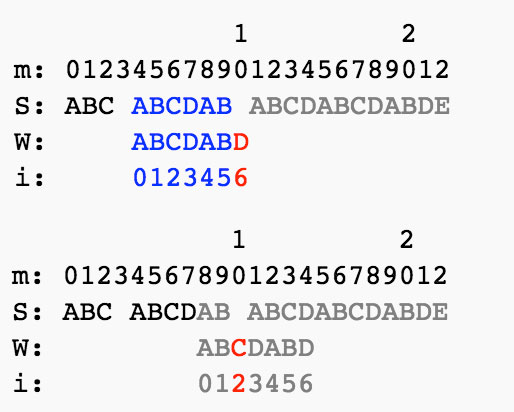
\includegraphics[scale=1.30]{kmp_presuffix}}
\caption{KMP example}
\label{fig:kmp_presuffix}
\end{figure}

\begin{figure}[hbtp]
\centering
\subfloat{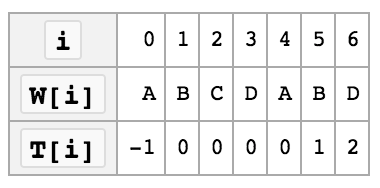
\includegraphics[scale=1.30]{kmp_table}}
\caption{Prefix-suffix table}
\label{fig:kmp_table}
\end{figure}
In table-building algorithm. $T[i]$ stores the NEXT prefix index $cnd$.\\
\\
Notice:
\begin{enumerate}
\item dummy at $T[0]=-1$.
\item three parts
\begin{enumerate}
\item matched
\item fall back
\item restart 
\end{enumerate}
\end{enumerate}
Code:
\begin{python}
# construct T
T = [0 for _ in xrange(ln+1)]
T[0] = -1
T[1] = 0
pos = 2
cnd = 0  
while pos <= ln:
    if needle[pos-1]==needle[cnd]:  # matched
        T[pos] = cnd+1
        cnd += 1
        pos += 1
    elif T[cnd]!=-1:  # fall back 
        cnd = T[cnd]
    else:  # restart 
        T[pos] = 0
        cnd = 0
        pos += 1

\end{python}


\subsection{Searching algorithm}
Notice:
\begin{enumerate}
\item index $i$ and $s$.
\item $T[i+1-1]$ for corresponding previous index in $T$ for current scanning index $i$. 
\item three parts:
\begin{enumerate}
\item matched
\item fall back
\item restart 
\end{enumerate}
\end{enumerate}
Code: 
\begin{python}
# search
i = 0  # index for needle 
j = 0  # index for haystack
while j+i < len(haystack):
    if needle[i] == haystack[j+i]:  # matched 
        i += 1
        if i == len(needle):
            return haystack[j:]
    else:
        if T[i] != -1:  # fall back
            j = j+i-T[i]
            i = T[i]
        else:  # restart
            j += 1
            i = 0

return None
\end{python}
\subsection{Applications}
\begin{enumerate}
\item Find needle in haystack. 
\item Shortest palindrome 
\end{enumerate}

